%%%%%%%%%%%%%%%%%%%%%%%%%%%%%%%%%%%%%%%%%%%%%%%%%%%%%%%%%%%%%%%%%%%%%%%%%%%%%%%%
\chapter{Экспериментальные исследования разработанной системы на Jetson Nano}
%%%%%%%%%%%%%%%%%%%%%%%%%%%%%%%%%%%%%%%%%%%%%%%%%%%%%%%%%%%%%%%%%%%%%%%%%%%%%%%%

%%%%%%%%%%%%%%%%%%%%%%%%%%%%%%%%%%%%%%%%%%%%%%%%%%%%%%%%%%%%%%%%%%%%%%%%%%%%%%%%
\section{Планирование экспериментальных исследований}
%%%%%%%%%%%%%%%%%%%%%%%%%%%%%%%%%%%%%%%%%%%%%%%%%%%%%%%%%%%%%%%%%%%%%%%%%%%%%%%%

В качестве эксперимента в данной работе представлены результаты запуска системы обнаружения типов транспортных средств с использованием разных моделей обнаружения, дообученных в разделе 2.2.2. Помимо этого, при тестировании используется модуль дополнительной классификации, влияние которого на общую производительность системы будет измерено в этом разделе.

В качестве оценки точности предлагается использовать метрику точности, описанную в разделе 2.2.2. Точность рассчитывается как для каждого класса объектов отдельно, так и для всех классов суммарно. Структура тестовой подвыборки для эксперимента описана в разделе 1.3.5.

Для проведения эксперимента по оценке точности на тестовой подвыборке был отключен модуль получения видеопотока с USB камеры, и вместо этого, кадры берутся из директории с тестовыми изображениями. После этого, результаты обнаружения (метки классов и координаты) записываются в отдельный файл, после чего выполняется расчет метрик точности.

После того как дообучение модели было завершено, необходимо выполнить конвертацию в формат TensorRT для запуска модели на Jetson. Для этого используется файл этапа обучения, который обычно состоит из трех файлов:

\fbox{%
  \parbox{\textwidth}{
    model.ckpt-\$\{CHECKPOINT\_NUMBER\}.data-00000-of-00001\\
    model.ckpt-\$\{CHECKPOINT\_NUMBER\}.index\\
	model.ckpt-\$\{CHECKPOINT\_NUMBER\}.meta
  }%
}

После того как был выбран файл, содержащий подходящий этап, необходимо выполнить команду:

\fbox{%
  \parbox{\textwidth}{
    python object\_detection\/export\_inference\_graph.py\\
    --input\_type=\$\{INPUT\_TYPE\}\\
    --pipeline\_config\_path=\$\{PIPELINE\_CONFIG\_PATH\}\\
    --trained\_checkpoint\_prefix=\$\{TRAINED\_CKPT\_PREFIX\}\\
    --output\_directory=\$\{EXPORT\_DIR\}
  }%
}

Результатом выполнения программы будут являться файлы:

%
\begin{itemize*}
  \item Фиксированный граф модели
  \item Конфигурационный файл модели
  \item Исходный файл этапа обучения модели
\end{itemize*}
%

Экспортированный файл модели далее необходимо передать в качестве входного аргумента в программе обнаружения объектов на Jetson. После того как будет выполнена десериализация модели в формат TensorRT Engine – начнется выполнение обнаружения. 

%%%%%%%%%%%%%%%%%%%%%%%%%%%%%%%%%%%%%%%%%%%%%%%%%%%%%%%%%%%%%%%%%%%%%%%%%%%%%%%%
\section{Метрики точности обнаружения и классификации}
%%%%%%%%%%%%%%%%%%%%%%%%%%%%%%%%%%%%%%%%%%%%%%%%%%%%%%%%%%%%%%%%%%%%%%%%%%%%%%%%

Анализ точности модели производился с помощью набора метрик, описанного в разделе 2.1. В частности, использовались такие оценки как:

%
\begin{itemize*}
  \item Средняя точность (AP) в зависимости от пересечения:
	%
	\begin{itemize*}
	  \item При пересечении областей не менее 50\%
	  \item При пересечении областей не менее 75\%
	  \item При пересечении областей не менее 90\%	  
	\end{itemize*}
	%
  \item Средняя точность (AP) в зависимости от размера области:
  	%
	\begin{itemize*}
	  \item При размере областей менее \(32^2\)
	  \item При размере областей более \(32^2\) но менее \(96^2\)
	  \item При размере областей более \(96^2\)
	\end{itemize*}
	%
  \item Средняя полнота (AR):
  	%
	\begin{itemize*}
	  \item При максимальном количестве объектов равным 1
	  \item При максимальном количестве объектов равным 10
	  \item При максимальном количестве объектов равным 100
	\end{itemize*}
	%
  \item Средняя полнота (AR) в зависимости от размера области:
  	%
	\begin{itemize*}
	  \item При размере областей менее \(32^2\)
	  \item При размере областей более \(32^2\) но менее \(96^2\)
	  \item При размере областей менее \(96^2\)
	\end{itemize*}
	%
\end{itemize*}
%

Для визуализации точности модели в данном разделе используется кривая точности и полноты. Данная кривая является методом оценки успешных обнаружений и показывает зависимость точности и полноты от различных порогов классификации. Общая площадь под кривой пропорциональна и высокой точности и высокой полноте, в то время как высокая точность соответствует низкой частоте ложно-положительных классификаций, а высокая полнота соответствует низкой частоте ложно-отрицательный классификаций. В случае если оба показателя имеют высокие значения, это означает что классификатор корректно определяет тип объекта, и находит большинство этих объектов в выборке.

%%%%%%%%%%%%%%%%%%%%%%%%%%%%%%%%%%%%%%%%%%%%%%%%%%%%%%%%%%%%%%%%%%%%%%%%%%%%%%%%
\section{Экспериментальные исследования системы с исходной моделью}
%%%%%%%%%%%%%%%%%%%%%%%%%%%%%%%%%%%%%%%%%%%%%%%%%%%%%%%%%%%%%%%%%%%%%%%%%%%%%%%%

Для оценки результатов дообучения модели и дополнительной классификации реализованной системы в этом разделе проведено тестирование исходной модели, взятой из репозитория TensorFlow. На таблице~\ref{tabular:tab_exp_1} приведены метрики точности и полноты обнаружения модели в зависимости от размера объектов и их количества на кадре.

\begin{table}[H]
	\def\arraystretch{1.3}
	\caption{Метрики точности исходной модели}
	\begin{center}
		\begin{tabular}{|l|c|}
			\hline
			Метрика & Значение\\  \hline			
			\(mAP^{50\%}\) & 0.53\\ \hline			
			\(mAP^{75\%}\) & 0.48\\ \hline
			\(mAP^{90\%}\) & 0.22\\ \hline
			\(mAP^{S<32}\) & 0.34\\ \hline
			\(mAP^{32<S<96}\) & 0.48\\ \hline
			\(mAP^{S>96}\) & 0.53\\ \hline
			\(mAP^{N=1}\) & 0.67\\ \hline
			\(mAP^{N<10}\) & 0.57\\ \hline
			\(mAP^{N<100}\) & 0.53\\ \hline
			\(mAP^{S<32}\) & 0.21\\ \hline
			\(mAP^{32<S<96}\) & 0.78\\ \hline
			\(mAP^{S>96}\) & 0.87\\ \hline			
		\end{tabular}
		\label{tabular:tab_exp_1}
	\end{center}
\end{table}

Для визуализации качества обнаружения объектов на рисунке~\ref{fig:image031} представлена зависимость точности и полноты обнаружения от порога классификации.

\begin{figure}[htbp]
\centering
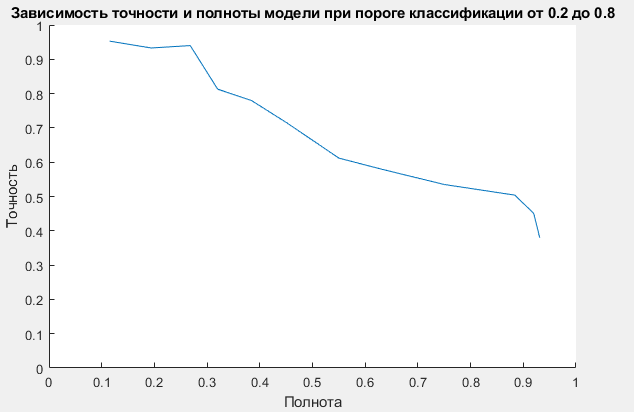
\includegraphics[width=0.85\textwidth]{image031.png}
\caption{Зависимость точности и полноты обнаружения модели от порога классификации}%
\label{fig:image031}
\end{figure}

Для оценки точности работы системы на рисунке~\ref{fig:image032} приведены метрики для каждого класса отдельно.

\begin{figure}[htbp]
\centering
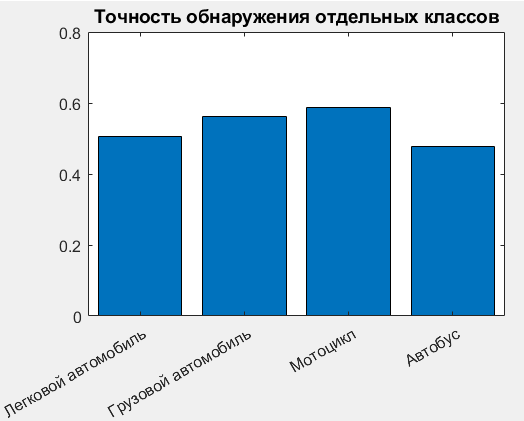
\includegraphics[width=0.85\textwidth]{image032.png}
\caption{Точность обнаружения по отдельным классам}%
\label{fig:image032}
\end{figure}

%%%%%%%%%%%%%%%%%%%%%%%%%%%%%%%%%%%%%%%%%%%%%%%%%%%%%%%%%%%%%%%%%%%%%%%%%%%%%%%%
\section{Экспериментальные исследования системы с дообученной моделью}
%%%%%%%%%%%%%%%%%%%%%%%%%%%%%%%%%%%%%%%%%%%%%%%%%%%%%%%%%%%%%%%%%%%%%%%%%%%%%%%%

Для оценки результатов дообучения в реализованной системе проведено тестирование модели, дообученной исключительно на метках классов «легковой автомобиль», «грузовой автомобиль», «мотоцикл», «трамвай» и «автобус». На таблице~\ref{tabular:tab_exp_2} приведены метрики точности и полноты обнаружения модели в зависимости от размера объектов и их количества на изображении.

\begin{table}[H]
	\def\arraystretch{1.3}
	\caption{Метрики точности дообученной модели}
	\begin{center}
		\begin{tabular}{|l|c|}
			\hline
			Метрика & Значение\\  \hline			
			\(mAP^{50\%}\) & 0.64\\ \hline			
			\(mAP^{75\%}\) & 0.59\\ \hline
			\(mAP^{90\%}\) & 0.27\\ \hline
			\(mAP^{S<32}\) & 0.39\\ \hline
			\(mAP^{32<S<96}\) & 0.57\\ \hline
			\(mAP^{S>96}\) & 0.64\\ \hline
			\(mAP^{N=1}\) & 0.75\\ \hline
			\(mAP^{N<10}\) & 0.63\\ \hline
			\(mAP^{N<100}\) & 0.64\\ \hline
			\(mAP^{S<32}\) & 0.32\\ \hline
			\(mAP^{32<S<96}\) & 0.83\\ \hline
			\(mAP^{S>96}\) & 0.88\\ \hline			
		\end{tabular}
		\label{tabular:tab_exp_2}
	\end{center}
\end{table}

Для визуализации качества обнаружения объектов на рисунке~\ref{fig:image033} представлена зависимость точности и полноты обнаружения от порога классификации.

\begin{figure}[htbp]
\centering
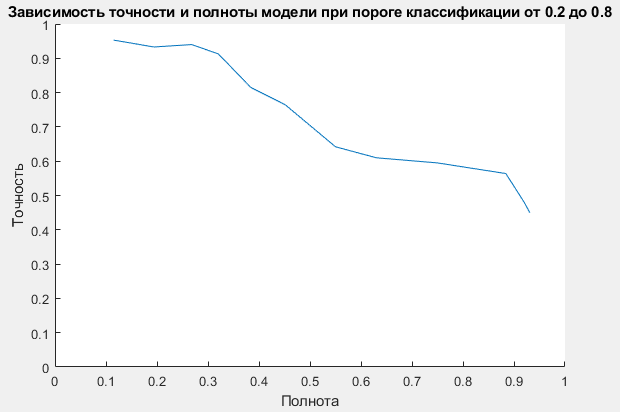
\includegraphics[width=0.85\textwidth]{image033.png}
\caption{Зависимость точности и полноты обнаружения модели от порога классификации}%
\label{fig:image033}
\end{figure}

Для оценки точности работы системы на рисунке~\ref{fig:image034} приведены метрики для каждого класса отдельно.

\begin{figure}[htbp]
\centering
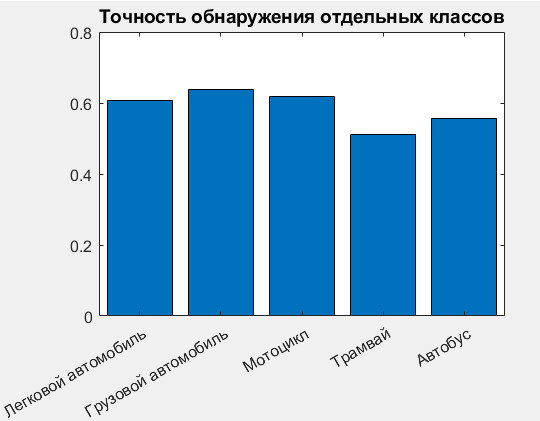
\includegraphics[width=0.85\textwidth]{image034.png}
\caption{Точность обнаружения по отдельным классам}%
\label{fig:image034}
\end{figure}

Для оценки результатов дообучения и дополнительной классификации в реализованной системе проведено тестирование модели, дообученной на метках классов «легковой автомобиль», «грузовой автомобиль», «мотоцикл», «трамвай», «автобус» и «троллейбус». На таблице~\ref{tabular:tab_exp_3} приведены метрики точности и полноты обнаружения модели в зависимости от размера объектов и их количества на изображении.

\begin{table}[H]
	\def\arraystretch{1.3}
	\caption{Метрики точности дообученной модели}
	\begin{center}
		\begin{tabular}{|l|c|}
			\hline
			Метрика & Значение\\  \hline			
			\(mAP^{50\%}\) & 0.48\\ \hline			
			\(mAP^{75\%}\) & 0.39\\ \hline
			\(mAP^{90\%}\) & 0.20\\ \hline
			\(mAP^{S<32}\) & 0.29\\ \hline
			\(mAP^{32<S<96}\) & 0.41\\ \hline
			\(mAP^{S>96}\) & 0.49\\ \hline
			\(mAP^{N=1}\) & 0.58\\ \hline
			\(mAP^{N<10}\) & 0.51\\ \hline
			\(mAP^{N<100}\) & 0.48\\ \hline
			\(mAP^{S<32}\) & 0.19\\ \hline
			\(mAP^{32<S<96}\) & 0.69\\ \hline
			\(mAP^{S>96}\) & 0.77\\ \hline			
		\end{tabular}
		\label{tabular:tab_exp_3}
	\end{center}
\end{table}

Для визуализации качества обнаружения объектов на рисунке~\ref{fig:image035} представлена зависимость точности и полноты обнаружения от порога классификации.

\begin{figure}[htbp]
\centering
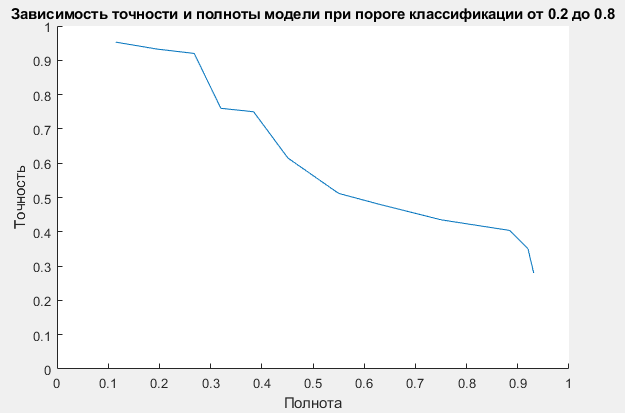
\includegraphics[width=0.85\textwidth]{image035.png}
\caption{Зависимость точности и полноты обнаружения модели от порога классификации}%
\label{fig:image035}
\end{figure}

Для оценки точности работы системы на рисунке~\ref{fig:image036} приведены метрики для каждого класса отдельно.

\begin{figure}[htbp]
\centering
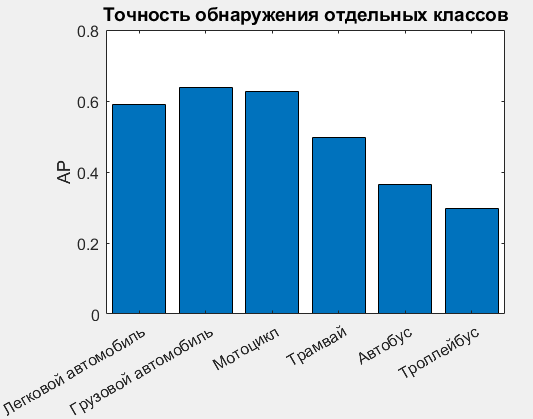
\includegraphics[width=0.85\textwidth]{image036.png}
\caption{Точность обнаружения по отдельным классам}%
\label{fig:image036}
\end{figure}

%%%%%%%%%%%%%%%%%%%%%%%%%%%%%%%%%%%%%%%%%%%%%%%%%%%%%%%%%%%%%%%%%%%%%%%%%%%%%%%%
\section{Экспериментальные исследования системы с дообученной моделью и дополнительной классификацией}
%%%%%%%%%%%%%%%%%%%%%%%%%%%%%%%%%%%%%%%%%%%%%%%%%%%%%%%%%%%%%%%%%%%%%%%%%%%%%%%%

Для оценки результатов дообучения и дополнительной классификации в реализованной системе проведено тестирование модели, дообученной на метках классов «легковой автомобиль», «грузовой автомобиль», «мотоцикл», «трамвай», «автобус» и «троллейбус». В данной конфигурации системы также присутствует модуль дополнительной классификации, основанный на фильтре Лапласа и ORB детекторе ключевых точек. На таблице~\ref{tabular:tab_exp_4} приведены метрики точности и полноты обнаружения модели в зависимости от размера объектов и их количества на изображении.

\begin{table}[H]
	\def\arraystretch{1.3}
	\caption{Метрики точности дообученной модели c дополнительной классификацией}
	\begin{center}
		\begin{tabular}{|l|c|}
			\hline
			Метрика & Значение\\  \hline			
			\(mAP^{50\%}\) & 0.63\\ \hline			
			\(mAP^{75\%}\) & 0.60\\ \hline
			\(mAP^{90\%}\) & 0.27\\ \hline
			\(mAP^{S<32}\) & 0.41\\ \hline
			\(mAP^{32<S<96}\) & 0.59\\ \hline
			\(mAP^{S>96}\) & 0.61\\ \hline
			\(mAP^{N=1}\) & 0.72\\ \hline
			\(mAP^{N<10}\) & 0.65\\ \hline
			\(mAP^{N<100}\) & 0.63\\ \hline
			\(mAP^{S<32}\) & 0.29\\ \hline
			\(mAP^{32<S<96}\) & 0.83\\ \hline
			\(mAP^{S>96}\) & 0.91\\ \hline			
		\end{tabular}
		\label{tabular:tab_exp_4}
	\end{center}
\end{table}

Для визуализации качества обнаружения объектов на рисунке~\ref{fig:image037} представлена зависимость точности и полноты от порога классификации.

\begin{figure}[htbp]
\centering
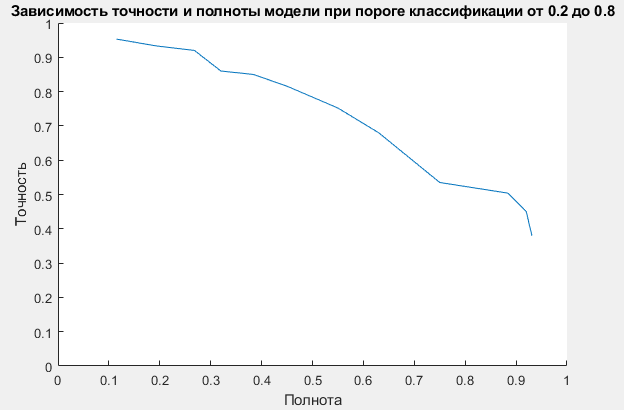
\includegraphics[width=0.85\textwidth]{image037.png}
\caption{Зависимость точности и полноты обнаружения модели от порога классификации}%
\label{fig:image037}
\end{figure}

Для оценки точности работы системы на рисунке~\ref{fig:image038} приведены метрики для каждого класса отдельно.

\begin{figure}[htbp]
\centering
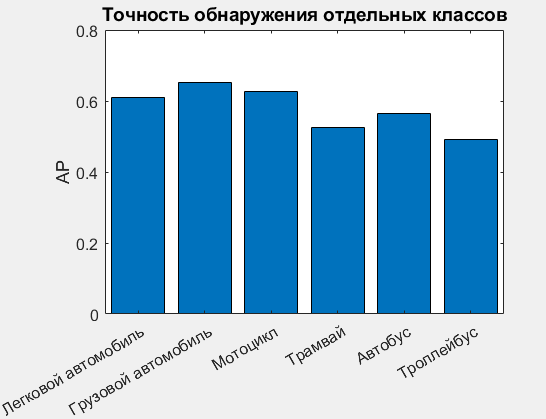
\includegraphics[width=0.85\textwidth]{image038.png}
\caption{Точность обнаружения по отдельным классам}%
\label{fig:image038}
\end{figure}

%%%%%%%%%%%%%%%%%%%%%%%%%%%%%%%%%%%%%%%%%%%%%%%%%%%%%%%%%%%%%%%%%%%%%%%%%%%%%%%%
\section{Выводы по разделу}
%%%%%%%%%%%%%%%%%%%%%%%%%%%%%%%%%%%%%%%%%%%%%%%%%%%%%%%%%%%%%%%%%%%%%%%%%%%%%%%%

В данном разделе были проведены опыты с различными конфигурациями системы обнаружения типов транспортных средств. Были представлены следующие конфигурации:

%
\begin{itemize*}
  \item С исходной моделью
  \item С дообученной моделью
  \item С дообученной моделью и дополнительной классификацией	  
\end{itemize*}
%
	
Для каждой из перечисленных выше конфигураций рассчитаны метрики точности и полноты, описывающие поведение системы в различных дорожных условиях, а также для различного количества объектов на кадре и их относительного размера. 

Для описания качества обнаружения и классификации в целом, представлены графики зависимости точности и полноты от порога классификации. Данная зависимость визуализирует количество успешных обнаружений и показывает зависимость точности и полноты от различных порогов классификации. Общая площадь под кривой пропорциональна и высокой точности и высокой полноте, в то время как высокая точность соответствует низкой частоте ложно-положительных классификаций, а высокая полнота соответствует низкой частоте ложно-отрицательный классификаций. 

Также, для визуализации сравнительных характеристик различных конфигураций системы на рисунке~\ref{fig:image039} представлен график зависимости средней точности (mAP) от конфигурации системы.

\begin{figure}[htbp]
\centering
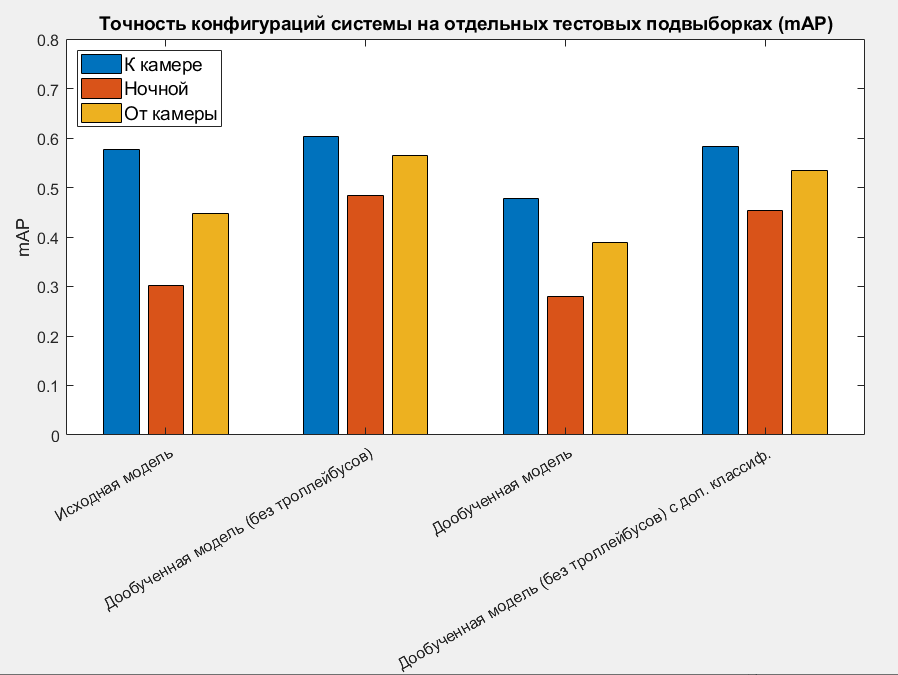
\includegraphics[width=0.85\textwidth]{image039.png}
\caption{Точность различных конфигураций системы}%
\label{fig:image039}
\end{figure}

Для оценки влияния используемого фильтра и детектора ключевых точек при дополнительной классификации на точность обнаружения транспортных средств с меткой «троллейбус» представлена таблица~\ref{tabular:tab_5} (значения указаны в метрике AP):

\begin{table}[H]
	\caption{Точность используемых комбинаций фильтра и дескриптора}
	\begin{center}
		\begin{tabular}{|l|c|c|c|}
			\hline
			 & ORB, AP & BRISK, AP & AKAZE, AP\\ \hline
			Без фильтра & 0.434 & 0.341 & 0.387\\ \hline
			Фильтр Лапласа & 0.502 & 0.310 & 0.469\\ \hline
			Алгоритм Кэнни (контуры) & 0.467 & 0.349 & 0.426\\ \hline			
		\end{tabular}
		\label{tabular:tab_5}
	\end{center}
\end{table}

В данной таблице указаны используемые комбинации фильтров и дескрипторов, а также соответствующая им точность обнаружения троллейбусов.

Дополнительно, представлена таблица~\ref{tabular:tab_6}, содержащая сведения о влиянии алгоритма дополнительной классификации на общее быстродействие системы.

\begin{table}[H]
	\caption{Точность используемых комбинаций фильтра и дескриптора}
	\begin{center}
		\begin{tabular}{|c|c|c|}
			\hline
			\multicolumn{2}{|c|}{Конфигурация} & FPS \\ \hline
			\multicolumn{2}{|c|}{Исходная система} & 22 \\ \hline
			\multirow{3}{*}{\begin{tabular}[c]{@{}c@{}}Система\\ с дополнительной\\ классификацией\end{tabular}}  & Без фильтра  & 19 \\ \cline{2-3} 
				 			   & Фильтр Лапласа  & 17 \\ \cline{2-3} 
							   & Алгоритм Кэнни  & 14 \\ \hline			
		\end{tabular}
		\label{tabular:tab_6}
	\end{center}
\end{table}

В таблице~\ref{tabular:tab_6} представлены использованные конфигурации системы и показатели их сравнительного быстродействия в режиме потоковой обработки кадров.












